% !Mode:: "TeX:UTF-8"

\chapter{小组成员信息}

小组成员信息及分工如表\ref{table::stuinfo1}

\begin{table}[htbp]
\centering
\caption{小组成员信息及分工}
\label{table::stuinfo1}
\begin{tabular}{|c|c|c|}
\hline
姓名& 学号& 分工安排\\
\hline
刘书裴& 3017218062& \multicolumn{1}{|m{7cm}|}{主持撰写研究汇报,制定研究计划;负责模型的设计、实现与优化。}\\
\hline
刘坤鑫& 3017218061& \multicolumn{1}{|m{7cm}|}{负责模型的测试与结果分析;精准评估模型存在的问题与不足;负责模型的设计、实现与优化。}\\
\hline
李喆  & 3017218198& \multicolumn{1}{|m{7cm}|}{负责研究报告、汇报PPT等文案的撰写与会议记录;负责模型的设计、实现与优化。}\\
\hline
芦源  & 3017210132& \multicolumn{1}{|m{7cm}|}{负责模型的设计、实现与优化;辅助完成项目中所需的其他算法。}\\
\hline
\end{tabular}
\end{table}

github提交进展如图\ref{fig::stuinfo1}。

\begin{figure}[htbp]
\centering
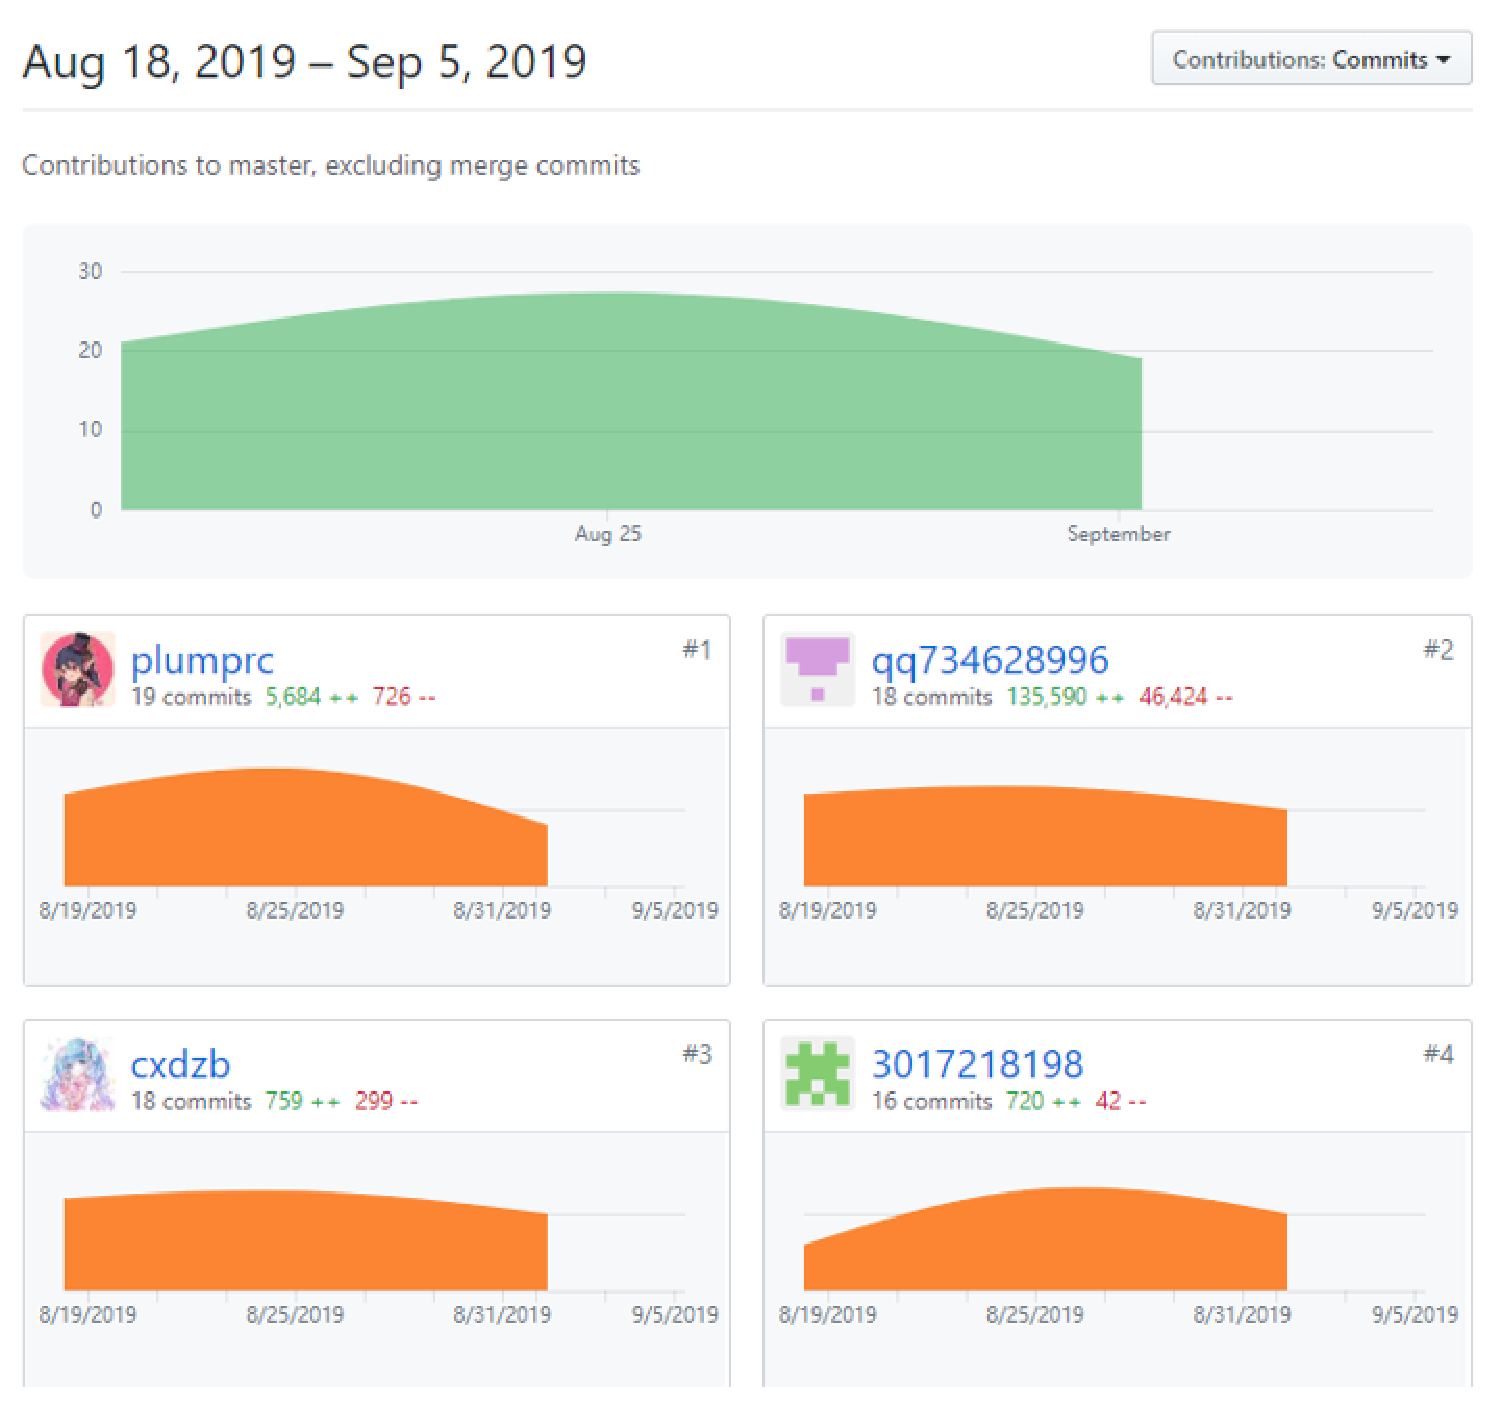
\includegraphics[width=0.8\linewidth]{body/stuinfo_pic/1}
\caption{github进展曲线图}
\label{fig::stuinfo1}
\end{figure}
